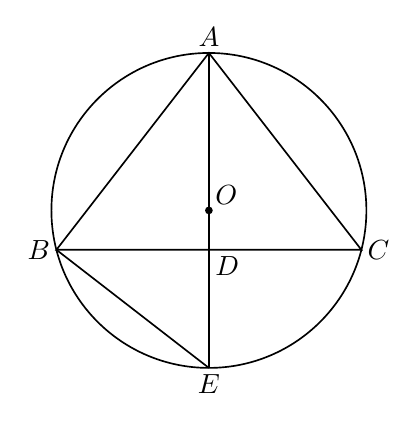
\begin{tikzpicture}[x=1cm,y=1cm,line width=.6pt,font=\normalsize]
\coordinate (O) at (0,0);
\coordinate (A) at (0,2);
\coordinate (E) at (0,-2);
\coordinate (D) at (0,-0.5);
\coordinate (B) at (-1.9365,-0.5);
\coordinate (C) at (1.9365,-0.5);
\draw (O) circle[radius=2cm];
\draw (A)--(B)--(C)--cycle;
\draw (A)--(E);
\draw (B)--(E);
\node[above=2pt,inner sep=0pt] at (A) {$A$};
\node[left=2pt,inner sep=0pt] at (B) {$B$};
\node[right=2pt,inner sep=0pt] at (C) {$C$};
\node[below=2pt,inner sep=0pt] at (E) {$E$};
\node[above right=2pt,inner sep=0pt] at (O) {$O$};
\node[below right=2pt,inner sep=0pt] at (D) {$D$};

% Explicit named circle-center points, painted after all region fills.
\fill (O) circle[radius=1.4pt];
\end{tikzpicture}
